\chapter{フローとカット - Flows and cuts}

この章では以下の2つの問題について解説します。

\begin{itemize}
\item \key{最大流の発見 - Finding a maximum flow}:
あるノードから他のノードに送ることができるフローの最大の量は?
\item \key{最小カットの発見 - Finding a minimum cut}:
グラフをに分割する辺のカットを最小にするには?
\end{itemize}

共通する前提は、2つの特殊なノードを含む重み付き有向グラフです。
ソースは入次辺を持たないノードで、
シンクは出次辺を持たないノードです。
次のグラフではノード1がソース、ノード6がシンクといえます。

\begin{center}
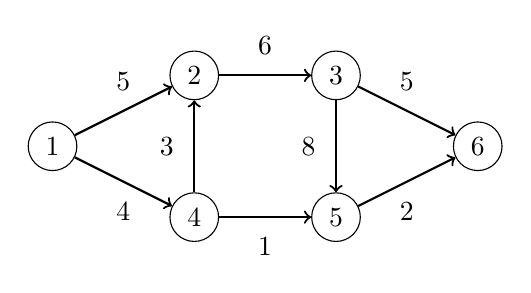
\begin{tikzpicture}[scale=0.9]
\node[draw, circle] (1) at (1,2) {$1$};
\node[draw, circle] (2) at (3,3) {$2$};
\node[draw, circle] (3) at (5,3) {$3$};
\node[draw, circle] (4) at (7,2) {$6$};
\node[draw, circle] (5) at (3,1) {$4$};
\node[draw, circle] (6) at (5,1) {$5$};
\path[draw,thick,->] (1) -- node[font=\small,label=5] {} (2);
\path[draw,thick,->] (2) -- node[font=\small,label=6] {} (3);
\path[draw,thick,->] (3) -- node[font=\small,label=5] {} (4);
\path[draw,thick,->] (1) -- node[font=\small,label=below:4] {} (5);
\path[draw,thick,->] (5) -- node[font=\small,label=below:1] {} (6);
\path[draw,thick,->] (6) -- node[font=\small,label=below:2] {} (4);
\path[draw,thick,<-] (2) -- node[font=\small,label=left:3] {} (5);
\path[draw,thick,->] (3) -- node[font=\small,label=left:8] {} (6);
\end{tikzpicture}
\end{center}

\subsubsection{最大流 - Maximum flow}

\index{フロー - flow}
\index{最大流 - maximum flow}

\key{最大流 - maximum flow}を求めるタスクは
ソースからシンクにできるだけ多くのフローを送ることです。
各エッジの重みは、そのエッジを通過できる最大のフローで容量と呼ばれます。
各中間ノードにおいて、流入するフローと流出するフローは等しくなければなりません。
次のグラフの例ではフローの最大サイズは7で、
そのフローをどのようにルーティングするかを示しています。

\begin{center}
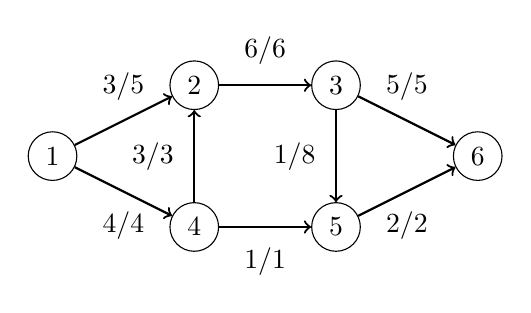
\begin{tikzpicture}[scale=0.9]
\node[draw, circle] (1) at (1,2) {$1$};
\node[draw, circle] (2) at (3,3) {$2$};
\node[draw, circle] (3) at (5,3) {$3$};
\node[draw, circle] (4) at (7,2) {$6$};
\node[draw, circle] (5) at (3,1) {$4$};
\node[draw, circle] (6) at (5,1) {$5$};
\path[draw,thick,->] (1) -- node[font=\small,label=3/5] {} (2);
\path[draw,thick,->] (2) -- node[font=\small,label=6/6] {} (3);
\path[draw,thick,->] (3) -- node[font=\small,label=5/5] {} (4);
\path[draw,thick,->] (1) -- node[font=\small,label=below:4/4] {} (5);
\path[draw,thick,->] (5) -- node[font=\small,label=below:1/1] {} (6);
\path[draw,thick,->] (6) -- node[font=\small,label=below:2/2] {} (4);
\path[draw,thick,<-] (2) -- node[font=\small,label=left:3/3] {} (5);
\path[draw,thick,->] (3) -- node[font=\small,label=left:1/8] {} (6);
\end{tikzpicture}
\end{center}

$v/k$という表記は、
$v$の流量のフローが$k$単位の容量を持つエッジを経由していることを意味します。
送信元が$3+4$のフローを送信し、
シンクが$5+2$ユ ニットのフローを受信するので、
このグラフのフローの大きさは7です。
このグラフではシンクにつながるエッジの総容量は7なので、
このフローが最大であることは容易に理解できるでしょう。

\subsubsection{最小カット - Minimum cut}

\index{カット - cut}
\index{最小カット - minimum cut}

\key{最小カット - minimum cut}問題とは、
グラフから辺の集合を削除していき、
削除後にソースからシンクへのパスが存在しなくなり、
削除した辺の総コストが最小となるようなものです。

例題のグラフのカットの最小サイズは7であり,辺$2 \rightarrow 3$
,$4 \rightarrow 5$を削除すれば良いです。

\begin{center}
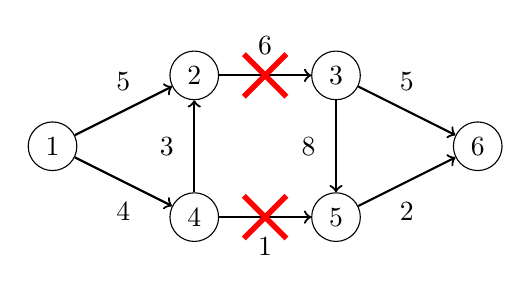
\begin{tikzpicture}[scale=0.9]
\node[draw, circle] (1) at (1,2) {$1$};
\node[draw, circle] (2) at (3,3) {$2$};
\node[draw, circle] (3) at (5,3) {$3$};
\node[draw, circle] (4) at (7,2) {$6$};
\node[draw, circle] (5) at (3,1) {$4$};
\node[draw, circle] (6) at (5,1) {$5$};
\path[draw,thick,->] (1) -- node[font=\small,label=5] {} (2);
\path[draw,thick,->] (2) -- node[font=\small,label=6] {} (3);
\path[draw,thick,->] (3) -- node[font=\small,label=5] {} (4);
\path[draw,thick,->] (1) -- node[font=\small,label=below:4] {} (5);
\path[draw,thick,->] (5) -- node[font=\small,label=below:1] {} (6);
\path[draw,thick,->] (6) -- node[font=\small,label=below:2] {} (4);
\path[draw,thick,<-] (2) -- node[font=\small,label=left:3] {} (5);
\path[draw,thick,->] (3) -- node[font=\small,label=left:8] {} (6);

\path[draw=red,thick,-,line width=2pt] (4-.3,3-.3) -- (4+.3,3+.3);
\path[draw=red,thick,-,line width=2pt] (4-.3,3+.3) -- (4+.3,3-.3);
\path[draw=red,thick,-,line width=2pt] (4-.3,1-.3) -- (4+.3,1+.3);
\path[draw=red,thick,-,line width=2pt] (4-.3,1+.3) -- (4+.3,1-.3);
\end{tikzpicture}
\end{center}

エッジを削除すると、ソースからシンクへのパスは存在しなくなります。
削除されたエッジの重みは$6$と$1$であるため、このカットの大きさは7です。
\\\\
上の例で最大流とカットの最小サイズが同じになりましたがこれは偶然ではありません。
最大フローと最小カットは常に同じ大きさです。
それでは、グラフの最大フローと最小カットを求めるための
フォード・ファルカーソンのアルゴリズムを見ていきます。
このアルゴリズムを理解することで、最大流と最小カットがなぜが等しくなるのか理解できるでしょう。

\section{フォード・ファルカーソンのアルゴリズム - Ford–Fulkerson algorithm}

\index{フォード・ファルカーソンのアルゴリズム - Ford–Fulkerson algorithm}

{フォード・ファルカーソンのアルゴリズム - Ford–Fulkerson algorithm} \cite{for56}
は、グラフの最大流量を求めるアルゴリズムです。
空のフローから始まり、各ステップではより多くのフローを生成するソースからシンクへの経路を見つけます。
最後に、これ以上フローを増やせなくなったとき、最大フローが発見されたと判定します。
このアルゴリズムは、元の辺がそれぞれ別の方向の逆辺を持つという、グラフの特殊な表現を使います。
各エッジの重みは、そのエッジを経由してどれだけ多くのフローをルーティングできるかを示します。
アルゴリズムの開始時点では、各オリジナルエッジの重みはエッジの容量に等しく、
各逆エッジの重みはゼロとしておきます。

\begin{samepage}
これを示したグラフは次のようになります。

\begin{center}
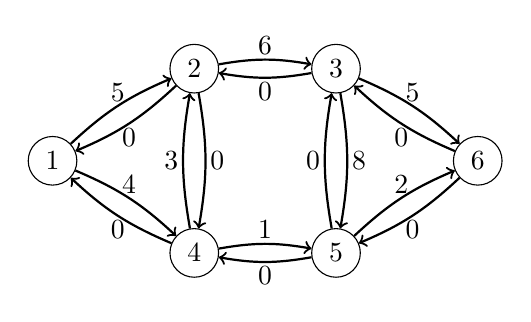
\begin{tikzpicture}[scale=0.9,label distance=-2mm]
\node[draw, circle] (1) at (1,1.3) {$1$};
\node[draw, circle] (2) at (3,2.6) {$2$};
\node[draw, circle] (3) at (5,2.6) {$3$};
\node[draw, circle] (4) at (7,1.3) {$6$};
\node[draw, circle] (5) at (3,0) {$4$};
\node[draw, circle] (6) at (5,0) {$5$};

\path[draw,thick,->] (1) edge [bend left=10] node[font=\small,label=5] {} (2);
\path[draw,thick,->] (2) edge [bend left=10] node[font=\small,label=below:0] {} (1);
\path[draw,thick,->] (2) edge [bend left=10] node[font=\small,label=6] {} (3);
\path[draw,thick,->] (3) edge [bend left=10] node[font=\small,label=below:0] {} (2);
\path[draw,thick,->] (3) edge [bend left=10] node[font=\small,label=5] {} (4);
\path[draw,thick,->] (4) edge [bend left=10] node[font=\small,label=below:0] {} (3);
\path[draw,thick,->] (1) edge [bend left=10] node[font=\small,label=4] {} (5);
\path[draw,thick,->] (5) edge [bend left=10] node[font=\small,label=below:0] {} (1);
\path[draw,thick,->] (5) edge [bend left=10] node[font=\small,label=1] {} (6);
\path[draw,thick,->] (6) edge [bend left=10] node[font=\small,label=below:0] {} (5);
\path[draw,thick,->] (6) edge [bend left=10] node[font=\small,label=2] {} (4);
\path[draw,thick,->] (4) edge [bend left=10] node[font=\small,label=below:0] {} (6);
\path[draw,thick,->] (5) edge [bend left=10] node[font=\small,label=left:3] {} (2);
\path[draw,thick,->] (2) edge [bend left=10] node[font=\small,label=right:0] {} (5);
\path[draw,thick,->] (3) edge [bend left=10] node[font=\small,label=right:8] {} (6);
\path[draw,thick,->] (6) edge [bend left=10] node[font=\small,label=left:0] {} (3);
\end{tikzpicture}
\end{center}
\end{samepage}

\subsubsection{アルゴリズムの説明 - Algorithm description}

この処理は複数のラウンドで構成されます。
各ラウンドで、アルゴリズムはソースからシンクへのパスを見つけ、
そのパス上の各エッジが正の重みを持つようにします。
複数の可能な経路がある場合は、そのうちのどれかを選択します。

例えば、次のようなパスを選択したとしましょう。

\begin{center}
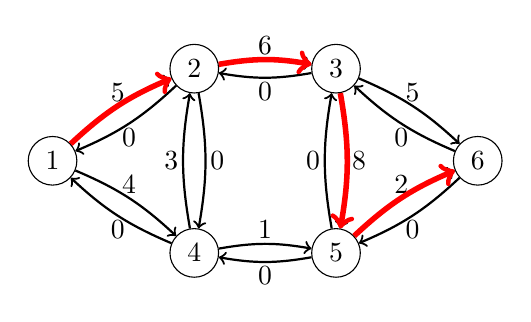
\begin{tikzpicture}[scale=0.9,label distance=-2mm]
\node[draw, circle] (1) at (1,1.3) {$1$};
\node[draw, circle] (2) at (3,2.6) {$2$};
\node[draw, circle] (3) at (5,2.6) {$3$};
\node[draw, circle] (4) at (7,1.3) {$6$};
\node[draw, circle] (5) at (3,0) {$4$};
\node[draw, circle] (6) at (5,0) {$5$};

\path[draw,thick,->] (1) edge [bend left=10] node[font=\small,label=5] {} (2);
\path[draw,thick,->] (2) edge [bend left=10] node[font=\small,label=below:0] {} (1);
\path[draw,thick,->] (2) edge [bend left=10] node[font=\small,label=6] {} (3);
\path[draw,thick,->] (3) edge [bend left=10] node[font=\small,label=below:0] {} (2);
\path[draw,thick,->] (3) edge [bend left=10] node[font=\small,label=5] {} (4);
\path[draw,thick,->] (4) edge [bend left=10] node[font=\small,label=below:0] {} (3);
\path[draw,thick,->] (1) edge [bend left=10] node[font=\small,label=4] {} (5);
\path[draw,thick,->] (5) edge [bend left=10] node[font=\small,label=below:0] {} (1);
\path[draw,thick,->] (5) edge [bend left=10] node[font=\small,label=1] {} (6);
\path[draw,thick,->] (6) edge [bend left=10] node[font=\small,label=below:0] {} (5);
\path[draw,thick,->] (6) edge [bend left=10] node[font=\small,label=2] {} (4);
\path[draw,thick,->] (4) edge [bend left=10] node[font=\small,label=below:0] {} (6);
\path[draw,thick,->] (5) edge [bend left=10] node[font=\small,label=left:3] {} (2);
\path[draw,thick,->] (2) edge [bend left=10] node[font=\small,label=right:0] {} (5);
\path[draw,thick,->] (3) edge [bend left=10] node[font=\small,label=right:8] {} (6);
\path[draw,thick,->] (6) edge [bend left=10] node[font=\small,label=left:0] {} (3);

\path[draw=red,thick,->,line width=2pt] (1) edge [bend left=10] (2);
\path[draw=red,thick,->,line width=2pt] (2) edge [bend left=10] (3);
\path[draw=red,thick,->,line width=2pt] (3) edge [bend left=10] (6);
\path[draw=red,thick,->,line width=2pt] (6) edge [bend left=10] (4);
\end{tikzpicture}
\end{center}

経路を選択した後、
フローはその経路に流せる最大の量である$x$単位で経路を増やします。
ここで、$x$は経路上の最小のエッジの重みとなります。
また、経路上の各辺の重みを$x$だけ減少させ、各逆辺の重みを$x$だけ増加させます。
上のパスでは、エッジの重みは5、6、8、2です。
最も小さい重みは2 なので、フローは2だけ増加し、新しいグラフは以下のようになります。

\begin{center}
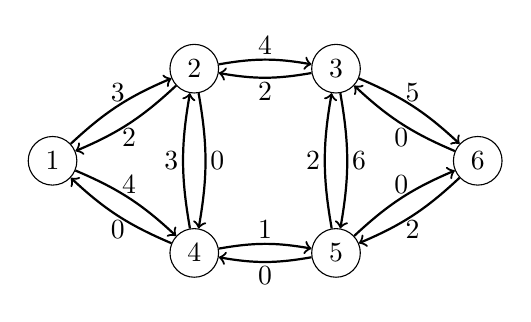
\begin{tikzpicture}[scale=0.9,label distance=-2mm]
\node[draw, circle] (1) at (1,1.3) {$1$};
\node[draw, circle] (2) at (3,2.6) {$2$};
\node[draw, circle] (3) at (5,2.6) {$3$};
\node[draw, circle] (4) at (7,1.3) {$6$};
\node[draw, circle] (5) at (3,0) {$4$};
\node[draw, circle] (6) at (5,0) {$5$};

\path[draw,thick,->] (1) edge [bend left=10] node[font=\small,label=3] {} (2);
\path[draw,thick,->] (2) edge [bend left=10] node[font=\small,label=below:2] {} (1);
\path[draw,thick,->] (2) edge [bend left=10] node[font=\small,label=4] {} (3);
\path[draw,thick,->] (3) edge [bend left=10] node[font=\small,label=below:2] {} (2);
\path[draw,thick,->] (3) edge [bend left=10] node[font=\small,label=5] {} (4);
\path[draw,thick,->] (4) edge [bend left=10] node[font=\small,label=below:0] {} (3);
\path[draw,thick,->] (1) edge [bend left=10] node[font=\small,label=4] {} (5);
\path[draw,thick,->] (5) edge [bend left=10] node[font=\small,label=below:0] {} (1);
\path[draw,thick,->] (5) edge [bend left=10] node[font=\small,label=1] {} (6);
\path[draw,thick,->] (6) edge [bend left=10] node[font=\small,label=below:0] {} (5);
\path[draw,thick,->] (6) edge [bend left=10] node[font=\small,label=0] {} (4);
\path[draw,thick,->] (4) edge [bend left=10] node[font=\small,label=below:2] {} (6);
\path[draw,thick,->] (5) edge [bend left=10] node[font=\small,label=left:3] {} (2);
\path[draw,thick,->] (2) edge [bend left=10] node[font=\small,label=right:0] {} (5);
\path[draw,thick,->] (3) edge [bend left=10] node[font=\small,label=right:6] {} (6);
\path[draw,thick,->] (6) edge [bend left=10] node[font=\small,label=left:2] {} (3);
\end{tikzpicture}
\end{center}

つまり、フローを増やすとそのエッジを通ることができるフローが減少するという操作です。
一方、フローを別の方法で流した方が有益であることが判明した場合、
グラフの逆エッジを使用してそのフローを後でキャンセル(減らす)ことができます。

このアルゴリズムは、
正の重みの辺を通るソースからシンクへの路が存在する限り、
操作を繰り返してフローを増加させます。
先ほどの直後では、次のような路が考えられる。

\begin{center}
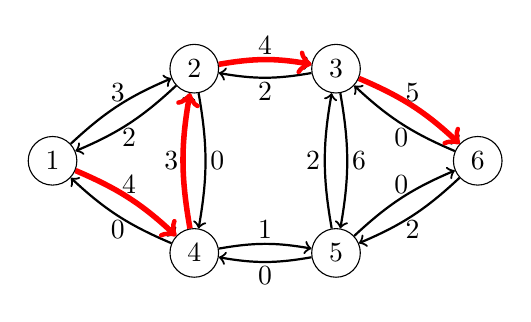
\begin{tikzpicture}[scale=0.9,label distance=-2mm]
\node[draw, circle] (1) at (1,1.3) {$1$};
\node[draw, circle] (2) at (3,2.6) {$2$};
\node[draw, circle] (3) at (5,2.6) {$3$};
\node[draw, circle] (4) at (7,1.3) {$6$};
\node[draw, circle] (5) at (3,0) {$4$};
\node[draw, circle] (6) at (5,0) {$5$};

\path[draw,thick,->] (1) edge [bend left=10] node[font=\small,label=3] {} (2);
\path[draw,thick,->] (2) edge [bend left=10] node[font=\small,label=below:2] {} (1);
\path[draw,thick,->] (2) edge [bend left=10] node[font=\small,label=4] {} (3);
\path[draw,thick,->] (3) edge [bend left=10] node[font=\small,label=below:2] {} (2);
\path[draw,thick,->] (3) edge [bend left=10] node[font=\small,label=5] {} (4);
\path[draw,thick,->] (4) edge [bend left=10] node[font=\small,label=below:0] {} (3);
\path[draw,thick,->] (1) edge [bend left=10] node[font=\small,label=4] {} (5);
\path[draw,thick,->] (5) edge [bend left=10] node[font=\small,label=below:0] {} (1);
\path[draw,thick,->] (5) edge [bend left=10] node[font=\small,label=1] {} (6);
\path[draw,thick,->] (6) edge [bend left=10] node[font=\small,label=below:0] {} (5);
\path[draw,thick,->] (6) edge [bend left=10] node[font=\small,label=0] {} (4);
\path[draw,thick,->] (4) edge [bend left=10] node[font=\small,label=below:2] {} (6);
\path[draw,thick,->] (5) edge [bend left=10] node[font=\small,label=left:3] {} (2);
\path[draw,thick,->] (2) edge [bend left=10] node[font=\small,label=right:0] {} (5);
\path[draw,thick,->] (3) edge [bend left=10] node[font=\small,label=right:6] {} (6);
\path[draw,thick,->] (6) edge [bend left=10] node[font=\small,label=left:2] {} (3);

\path[draw=red,thick,->,line width=2pt] (1) edge [bend left=10] (5);
\path[draw=red,thick,->,line width=2pt] (5) edge [bend left=10] (2);
\path[draw=red,thick,->,line width=2pt] (2) edge [bend left=10] (3);
\path[draw=red,thick,->,line width=2pt] (3) edge [bend left=10] (4);
\end{tikzpicture}
\end{center}

このパスの最小の重さは3なので、このパスによってフローは3増加し、
パス処理後の総フローは5となります。

\begin{samepage}
新しいグラフは以下のようになります。

\begin{center}
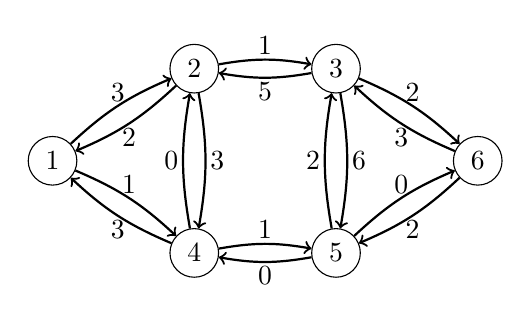
\begin{tikzpicture}[scale=0.9,label distance=-2mm]
\node[draw, circle] (1) at (1,1.3) {$1$};
\node[draw, circle] (2) at (3,2.6) {$2$};
\node[draw, circle] (3) at (5,2.6) {$3$};
\node[draw, circle] (4) at (7,1.3) {$6$};
\node[draw, circle] (5) at (3,0) {$4$};
\node[draw, circle] (6) at (5,0) {$5$};

\path[draw,thick,->] (1) edge [bend left=10] node[font=\small,label=3] {} (2);
\path[draw,thick,->] (2) edge [bend left=10] node[font=\small,label=below:2] {} (1);
\path[draw,thick,->] (2) edge [bend left=10] node[font=\small,label=1] {} (3);
\path[draw,thick,->] (3) edge [bend left=10] node[font=\small,label=below:5] {} (2);
\path[draw,thick,->] (3) edge [bend left=10] node[font=\small,label=2] {} (4);
\path[draw,thick,->] (4) edge [bend left=10] node[font=\small,label=below:3] {} (3);
\path[draw,thick,->] (1) edge [bend left=10] node[font=\small,label=1] {} (5);
\path[draw,thick,->] (5) edge [bend left=10] node[font=\small,label=below:3] {} (1);
\path[draw,thick,->] (5) edge [bend left=10] node[font=\small,label=1] {} (6);
\path[draw,thick,->] (6) edge [bend left=10] node[font=\small,label=below:0] {} (5);
\path[draw,thick,->] (6) edge [bend left=10] node[font=\small,label=0] {} (4);
\path[draw,thick,->] (4) edge [bend left=10] node[font=\small,label=below:2] {} (6);
\path[draw,thick,->] (5) edge [bend left=10] node[font=\small,label=left:0] {} (2);
\path[draw,thick,->] (2) edge [bend left=10] node[font=\small,label=right:3] {} (5);
\path[draw,thick,->] (3) edge [bend left=10] node[font=\small,label=right:6] {} (6);
\path[draw,thick,->] (6) edge [bend left=10] node[font=\small,label=left:2] {} (3);
\end{tikzpicture}
\end{center}
\end{samepage}

最大流量に達するまで、まだ2ラウンド操作できます。
例えば、
$1 \rightarrow 2 \rightarrow 3 \rightarrow 6$ と
$1 \rightarrow 4 \rightarrow 5 \rightarrow 3 \rightarrow 6$ という経路です。
どちらの経路もフローを 1 増加させ、最終的なグラフは以下のようになります。

\begin{center}
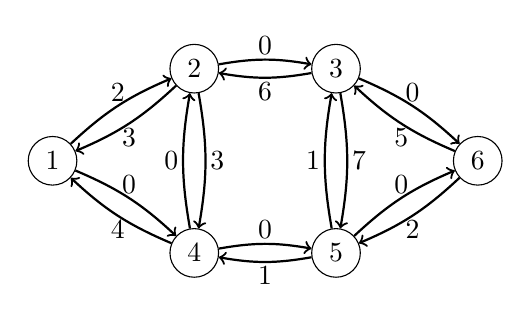
\begin{tikzpicture}[scale=0.9,label distance=-2mm]
\node[draw, circle] (1) at (1,1.3) {$1$};
\node[draw, circle] (2) at (3,2.6) {$2$};
\node[draw, circle] (3) at (5,2.6) {$3$};
\node[draw, circle] (4) at (7,1.3) {$6$};
\node[draw, circle] (5) at (3,0) {$4$};
\node[draw, circle] (6) at (5,0) {$5$};

\path[draw,thick,->] (1) edge [bend left=10] node[font=\small,label=2] {} (2);
\path[draw,thick,->] (2) edge [bend left=10] node[font=\small,label=below:3] {} (1);
\path[draw,thick,->] (2) edge [bend left=10] node[font=\small,label=0] {} (3);
\path[draw,thick,->] (3) edge [bend left=10] node[font=\small,label=below:6] {} (2);
\path[draw,thick,->] (3) edge [bend left=10] node[font=\small,label=0] {} (4);
\path[draw,thick,->] (4) edge [bend left=10] node[font=\small,label=below:5] {} (3);
\path[draw,thick,->] (1) edge [bend left=10] node[font=\small,label=0] {} (5);
\path[draw,thick,->] (5) edge [bend left=10] node[font=\small,label=below:4] {} (1);
\path[draw,thick,->] (5) edge [bend left=10] node[font=\small,label=0] {} (6);
\path[draw,thick,->] (6) edge [bend left=10] node[font=\small,label=below:1] {} (5);
\path[draw,thick,->] (6) edge [bend left=10] node[font=\small,label=0] {} (4);
\path[draw,thick,->] (4) edge [bend left=10] node[font=\small,label=below:2] {} (6);
\path[draw,thick,->] (5) edge [bend left=10] node[font=\small,label=left:0] {} (2);
\path[draw,thick,->] (2) edge [bend left=10] node[font=\small,label=right:3] {} (5);
\path[draw,thick,->] (3) edge [bend left=10] node[font=\small,label=right:7] {} (6);
\path[draw,thick,->] (6) edge [bend left=10] node[font=\small,label=left:1] {} (3);
\end{tikzpicture}
\end{center}


ソースからシンクまで正のエッジ重みを持つパスが存在しないため、新しい路はつくれません。
したがって、アルゴリズムは終了し、最大フローは7となりました。

\subsubsection{パスの検索 - Finding paths}

フォード・ファルカーソン アルゴリズムでは、
流量を増加させる経路をどのように選択すべきかは指定されていません。
どのような路を選んでも、アルゴリズムは遅かれ早かれ収束し、
正しく最大流量を求めることができる。
ただし、経路の選び方次第で効率は変わってきます。

経路を見つける簡単な方法は深さ優先探索です。
通常、これはうまくいきますが、最悪のケースでは各パスがフローを1だけ増加させ、アルゴリズムは遅く動作します。
そこで、次のような手法を用いることで効率的にパスを選択できます。

\index{エドモンズ・カープのアルゴリズム - Edmonds–Karp algorithm}

\key{エドモンズ・カープのアルゴリズム - Edmonds–Karp algorithm} \cite{edm72}
は、なるべく辺の数ができるだけ少なくなるようにパスを選択します。
これは、パスには幅優先探索を用いることで実現できます。
これにより、フローが迅速に増加することが保証され、
このアルゴリズムの時間複雑性は $O(m^2 n)$であることが証明され得る。


\index{スケーリングアルゴリズム - scaling algorithm}\cite{ahu91} は
深さ優先探索により、選択する各辺の重みが少なくとも閾値以上である経路を見つけるものである。
初期状態では、閾値はある大きな数、例えばグラフの全てのエッジ重みの和からスタートします。
パスが見つからないときは閾値を2で割ります。
このアルゴリズムの時間計算量は$O(m^2 \log c)$であり、ここでcは初期の閾値です。
深さ優先探索で経路を見つけることができるため、
スケーリングアルゴリズムの方が実装が簡単です。

どちらのアルゴリズムも、
プログラミングコンテストでよく出題されるような問題には十分です。

\subsubsection{最小カット - Minimum cuts}

\index{最小カット - minimum cut}

フォード・ファルカーソンアルゴリズムが最大流量を求めると、
最小カットも求められることがわかっています。
正の重みのエッジを使ってソースから到達可能なノードのある集合を$A$とします。

例のグラフでは、Aにはノード1、2、4が含まれる。

\begin{center}
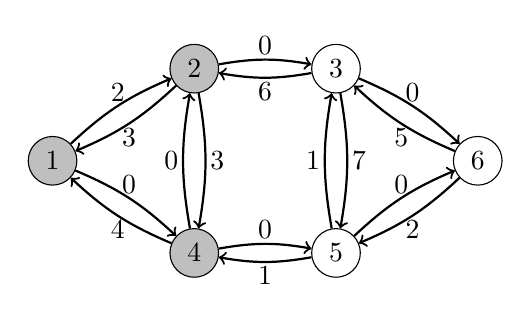
\begin{tikzpicture}[scale=0.9,label distance=-2mm]
\node[draw, circle,fill=lightgray] (1) at (1,1.3) {$1$};
\node[draw, circle,fill=lightgray] (2) at (3,2.6) {$2$};
\node[draw, circle] (3) at (5,2.6) {$3$};
\node[draw, circle] (4) at (7,1.3) {$6$};
\node[draw, circle,fill=lightgray] (5) at (3,0) {$4$};
\node[draw, circle] (6) at (5,0) {$5$};

\path[draw,thick,->] (1) edge [bend left=10] node[font=\small,label=2] {} (2);
\path[draw,thick,->] (2) edge [bend left=10] node[font=\small,label=below:3] {} (1);
\path[draw,thick,->] (2) edge [bend left=10] node[font=\small,label=0] {} (3);
\path[draw,thick,->] (3) edge [bend left=10] node[font=\small,label=below:6] {} (2);
\path[draw,thick,->] (3) edge [bend left=10] node[font=\small,label=0] {} (4);
\path[draw,thick,->] (4) edge [bend left=10] node[font=\small,label=below:5] {} (3);
\path[draw,thick,->] (1) edge [bend left=10] node[font=\small,label=0] {} (5);
\path[draw,thick,->] (5) edge [bend left=10] node[font=\small,label=below:4] {} (1);
\path[draw,thick,->] (5) edge [bend left=10] node[font=\small,label=0] {} (6);
\path[draw,thick,->] (6) edge [bend left=10] node[font=\small,label=below:1] {} (5);
\path[draw,thick,->] (6) edge [bend left=10] node[font=\small,label=0] {} (4);
\path[draw,thick,->] (4) edge [bend left=10] node[font=\small,label=below:2] {} (6);
\path[draw,thick,->] (5) edge [bend left=10] node[font=\small,label=left:0] {} (2);
\path[draw,thick,->] (2) edge [bend left=10] node[font=\small,label=right:3] {} (5);
\path[draw,thick,->] (3) edge [bend left=10] node[font=\small,label=right:7] {} (6);
\path[draw,thick,->] (6) edge [bend left=10] node[font=\small,label=left:1] {} (3);
\end{tikzpicture}
\end{center}

最小カットは元のグラフの、A内のあるノードから始まり、A以外のノードで終わり、
その容量は最大フローで完全に使われる辺で構成されています。
上のグラフでは、$2 \rightarrow 3$ と $4 \rightarrow 5$がそのような辺で、
最小カット$6+1=7$に 相当する。

アルゴリズムが生成するフローはなぜ最大流となり、カットはなぜ最小となるのでしょうか?
その理由は、グラフのカットの重さよりも大きなサイズのフローというのは含むことができないからです。
したがって、フローとカットが同じ大きさであれば 、常に最大フローと最小カットとなります。

例としてソースが$A$に属し、シンクが$B$に属し、
その集合の間にいくつかのエッジが存在するようなグラフのカットを考えることにしよう。

\begin{center}
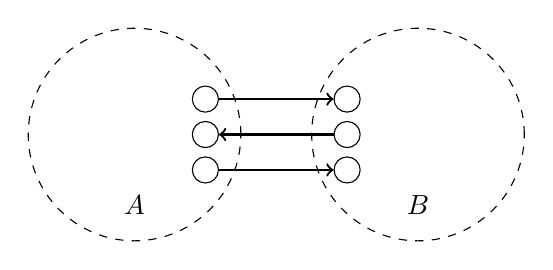
\begin{tikzpicture}[scale=0.9]
\draw[dashed] (-2,0) circle (1.5);
\draw[dashed] (2,0) circle (1.5);

\node at (-2,-1) {$A$};
\node at (2,-1) {$B$};

\node[draw, circle] (1) at (-1,0.5) {};
\node[draw, circle] (2) at (-1,0) {};
\node[draw, circle] (3) at (-1,-0.5) {};
\node[draw, circle] (4) at (1,0.5) {};
\node[draw, circle] (5) at (1,0) {};
\node[draw, circle] (6) at (1,-0.5) {};

\path[draw,thick,->] (1) -- (4);
\path[draw,thick,->] (5) -- (2);
\path[draw,thick,->] (3) -- (6);

\end{tikzpicture}
\end{center}

カットのサイズとは$A$から$B$に進む辺の合計です。
これは、グラフ内のフローが$A$から$B$に流れているということです。
したがって、最大流の大きさは、グラフのどのカットの大きさよりも小さいか等しくなることは明らかです。

一方、フォード・ファルカーソン法では、
グラフのカットのサイズとちょうど同じ大きさのフローが生成されます。
したがって、フローは最大フローでな ければならず、カットは最小カットでなければならない。


\section{素なパス - Disjoint paths}

多くのグラフ問題は、最大流問題に還元することで解くことができます。1つの例をあげます。

ソースとシンクを持つ有向グラフが与えられ、
ソースからシンクへの素なパスの最大数を見つけてください。

\subsubsection{辺素なパス}

まず、ソースからシンクまでの辺素なパスの最大数を求めましょう。
つまり、各エッジが最大でも1つの経路に現れるような経路の集合を構成することである。

例えば、次のようなグラフを考えてみましょう。

\begin{center}
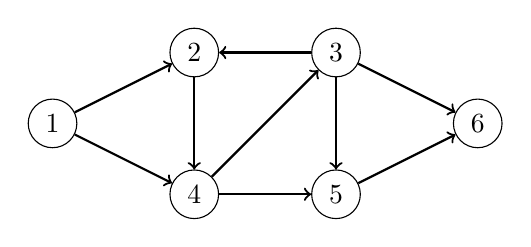
\begin{tikzpicture}[scale=0.9]
\node[draw, circle] (1) at (1,2) {$1$};
\node[draw, circle] (2) at (3,3) {$2$};
\node[draw, circle] (3) at (5,3) {$3$};
\node[draw, circle] (4) at (3,1) {$4$};
\node[draw, circle] (5) at (5,1) {$5$};
\node[draw, circle] (6) at (7,2) {$6$};
\path[draw,thick,->] (1) -- (2);
\path[draw,thick,->] (1) -- (4);
\path[draw,thick,->] (2) -- (4);
\path[draw,thick,->] (3) -- (2);
\path[draw,thick,->] (3) -- (5);
\path[draw,thick,->] (3) -- (6);
\path[draw,thick,->] (4) -- (3);
\path[draw,thick,->] (4) -- (5);
\path[draw,thick,->] (5) -- (6);
\end{tikzpicture}
\end{center}

このグラフにおいて,辺素なパスの最大数は2で、
$1 \rightarrow 2 \rightarrow 4 \rightarrow 3 \rightarrow 6$
と $1 \rightarrow 4 \rightarrow 5 \rightarrow 6$
を以下のように選ぶことができる.

\begin{center}
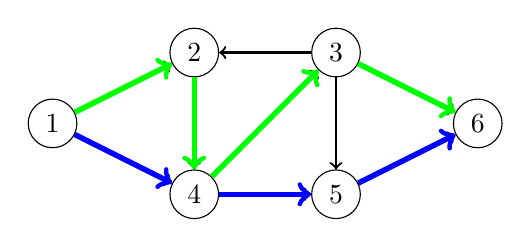
\begin{tikzpicture}[scale=0.9]
\node[draw, circle] (1) at (1,2) {$1$};
\node[draw, circle] (2) at (3,3) {$2$};
\node[draw, circle] (3) at (5,3) {$3$};
\node[draw, circle] (4) at (3,1) {$4$};
\node[draw, circle] (5) at (5,1) {$5$};
\node[draw, circle] (6) at (7,2) {$6$};
\path[draw,thick,->] (1) -- (2);
\path[draw,thick,->] (1) -- (4);
\path[draw,thick,->] (2) -- (4);
\path[draw,thick,->] (3) -- (2);
\path[draw,thick,->] (3) -- (5);
\path[draw,thick,->] (3) -- (6);
\path[draw,thick,->] (4) -- (3);
\path[draw,thick,->] (4) -- (5);
\path[draw,thick,->] (5) -- (6);

\path[draw=green,thick,->,line width=2pt] (1) -- (2);
\path[draw=green,thick,->,line width=2pt] (2) -- (4);
\path[draw=green,thick,->,line width=2pt] (4) -- (3);
\path[draw=green,thick,->,line width=2pt] (3) -- (6);

\path[draw=blue,thick,->,line width=2pt] (1) -- (4);
\path[draw=blue,thick,->,line width=2pt] (4) -- (5);
\path[draw=blue,thick,->,line width=2pt] (5) -- (6);
\end{tikzpicture}
\end{center}

各エッジの容量を1とすると、
辺素なパスの最大数はグラフの最大フロ ーに等しいことが判明しました。
最大流が構成された後の辺素なパスの経路は、
ソースからシンクへの経路を貪欲にたどることで見つけることができます。

\subsubsection{ノードが素なパス - Node-disjoint paths}

では別の問題として、ソースからシンクまでのノードが素なパスの最大数を求めます。
ここで、ソースとシンクは複数回登場しても良いです。

このグラフの場合は1となります。

\begin{center}
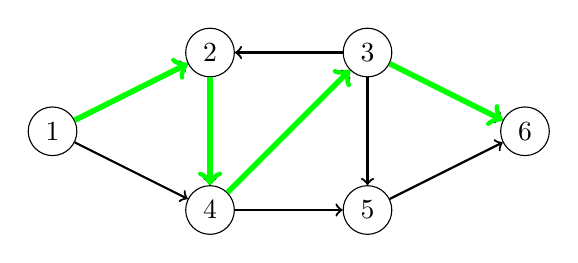
\begin{tikzpicture}
\node[draw, circle] (1) at (1,2) {$1$};
\node[draw, circle] (2) at (3,3) {$2$};
\node[draw, circle] (3) at (5,3) {$3$};
\node[draw, circle] (4) at (3,1) {$4$};
\node[draw, circle] (5) at (5,1) {$5$};
\node[draw, circle] (6) at (7,2) {$6$};
\path[draw,thick,->] (1) -- (2);
\path[draw,thick,->] (1) -- (4);
\path[draw,thick,->] (2) -- (4);
\path[draw,thick,->] (3) -- (2);
\path[draw,thick,->] (3) -- (5);
\path[draw,thick,->] (3) -- (6);
\path[draw,thick,->] (4) -- (3);
\path[draw,thick,->] (4) -- (5);
\path[draw,thick,->] (5) -- (6);

\path[draw=green,thick,->,line width=2pt] (1) -- (2);
\path[draw=green,thick,->,line width=2pt] (2) -- (4);
\path[draw=green,thick,->,line width=2pt] (4) -- (3);
\path[draw=green,thick,->,line width=2pt] (3) -- (6);
\end{tikzpicture}
\end{center}

この問題も最大流問題とすることができます。
各ノードは最大でも1つの経路にしか現れないので、
ノードを通過する流れを制限しなければなりません。
このための標準的な方法は、各ノードを2つのノードに分割し,
最初のノードは元のノードの入次辺を持ち,2番目のノードが出次辺を持つようにします。
そして、最初のノードから2番目のノードに向かう新しいエッジが存在するようにします。

この例では、グラフは次のようになる。

In our example, the graph becomes as follows:
\begin{center}
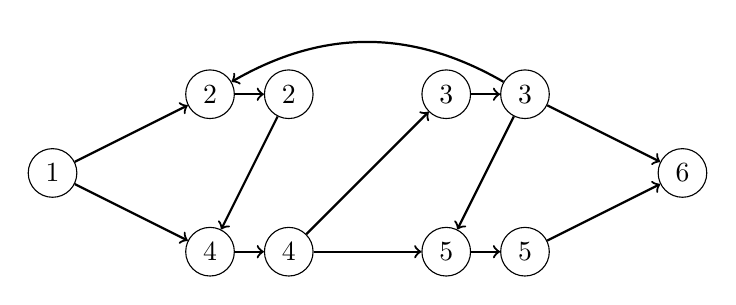
\begin{tikzpicture}
\node[draw, circle] (1) at (1,2) {$1$};

\node[draw, circle] (2a) at (3,3) {$2$};
\node[draw, circle] (3a) at (6,3) {$3$};
\node[draw, circle] (4a) at (3,1) {$4$};
\node[draw, circle] (5a) at (6,1) {$5$};

\node[draw, circle] (2b) at (4,3) {$2$};
\node[draw, circle] (3b) at (7,3) {$3$};
\node[draw, circle] (4b) at (4,1) {$4$};
\node[draw, circle] (5b) at (7,1) {$5$};

\node[draw, circle] (6) at (9,2) {$6$};

\path[draw,thick,->] (2a) -- (2b);
\path[draw,thick,->] (3a) -- (3b);
\path[draw,thick,->] (4a) -- (4b);
\path[draw,thick,->] (5a) -- (5b);

\path[draw,thick,->] (1) -- (2a);
\path[draw,thick,->] (1) -- (4a);
\path[draw,thick,->] (2b) -- (4a);
\path[draw,thick,->] (3b) edge [bend right=30] (2a);
\path[draw,thick,->] (3b) -- (5a);
\path[draw,thick,->] (3b) -- (6);
\path[draw,thick,->] (4b) -- (3a);
\path[draw,thick,->] (4b) -- (5a);
\path[draw,thick,->] (5b) -- (6);
\end{tikzpicture}
\end{center}

最大流は以下のようになります。

\begin{center}
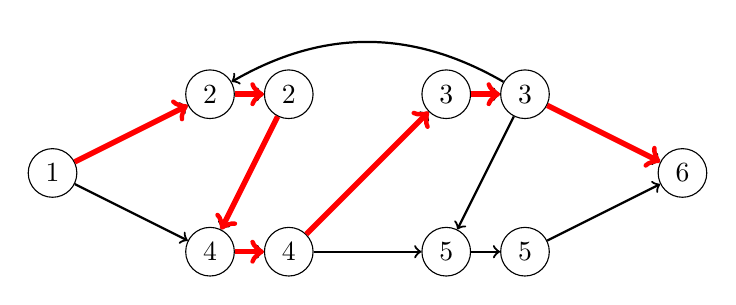
\begin{tikzpicture}
\node[draw, circle] (1) at (1,2) {$1$};

\node[draw, circle] (2a) at (3,3) {$2$};
\node[draw, circle] (3a) at (6,3) {$3$};
\node[draw, circle] (4a) at (3,1) {$4$};
\node[draw, circle] (5a) at (6,1) {$5$};

\node[draw, circle] (2b) at (4,3) {$2$};
\node[draw, circle] (3b) at (7,3) {$3$};
\node[draw, circle] (4b) at (4,1) {$4$};
\node[draw, circle] (5b) at (7,1) {$5$};

\node[draw, circle] (6) at (9,2) {$6$};

\path[draw,thick,->] (2a) -- (2b);
\path[draw,thick,->] (3a) -- (3b);
\path[draw,thick,->] (4a) -- (4b);
\path[draw,thick,->] (5a) -- (5b);

\path[draw,thick,->] (1) -- (2a);
\path[draw,thick,->] (1) -- (4a);
\path[draw,thick,->] (2b) -- (4a);
\path[draw,thick,->] (3b) edge [bend right=30] (2a);
\path[draw,thick,->] (3b) -- (5a);
\path[draw,thick,->] (3b) -- (6);
\path[draw,thick,->] (4b) -- (3a);
\path[draw,thick,->] (4b) -- (5a);
\path[draw,thick,->] (5b) -- (6);

\path[draw=red,thick,->,line width=2pt] (1) -- (2a);
\path[draw=red,thick,->,line width=2pt] (2a) -- (2b);
\path[draw=red,thick,->,line width=2pt] (2b) -- (4a);
\path[draw=red,thick,->,line width=2pt] (4a) -- (4b);
\path[draw=red,thick,->,line width=2pt] (4b) -- (3a);
\path[draw=red,thick,->,line width=2pt] (3a) -- (3b);
\path[draw=red,thick,->,line width=2pt] (3b) -- (6);
\end{tikzpicture}
\end{center}

この最大流は1となり、このため、ノードが素な経路の数は1となります。

\section{最大マッチング - Maximum matchings}

\index{マッチング - matching}
\index{最大マッチング - maximum matching}

\key{最大マッチング問題 - maximum matching}は、
無向グラフにおいて、各ノードの集合のペアを考え、
各ノードが最大1つのペアに属するような、
最大サイズのノードペアの集合を求める問題です。

一般的なグラフでも最大マッチングを求める多項式アルゴリズムがあるが\cite{edm65}、
そのようなアルゴリズムは複雑で、
プログラミングコンテストで見られることはほぼありません。
しかし、二部グラフでは、最大マッチング問題は最大フロー問題に還元できます。

\subsubsection{最大マッチングの検出 - Finding maximum matchings}

二部グラフのノードは常に2つのグループに分けられ、
グラフのすべてのエッジが左のグループから右のグループに辺が張られています。
例えば、次の二部グラフでは、グループは $\{1,2,3,4\}$ と $\{5,6,7,8\}$です。

\begin{center}
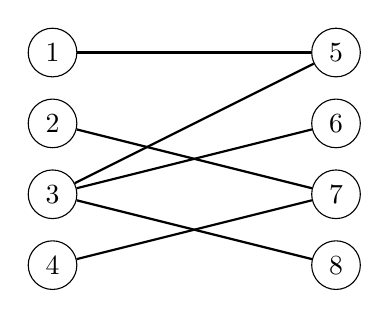
\begin{tikzpicture}[scale=0.60]
\node[draw, circle] (1) at (2,4.5) {1};
\node[draw, circle] (2) at (2,3) {2};
\node[draw, circle] (3) at (2,1.5) {3};
\node[draw, circle] (4) at (2,0) {4};
\node[draw, circle] (5) at (8,4.5) {5};
\node[draw, circle] (6) at (8,3) {6};
\node[draw, circle] (7) at (8,1.5) {7};
\node[draw, circle] (8) at (8,0) {8};

\path[draw,thick,-] (1) -- (5);
\path[draw,thick,-] (2) -- (7);
\path[draw,thick,-] (3) -- (5);
\path[draw,thick,-] (3) -- (6);
\path[draw,thick,-] (3) -- (8);
\path[draw,thick,-] (4) -- (7);
\end{tikzpicture}
\end{center}
このグラフの最大マッチングの大きさは3です。
\begin{center}
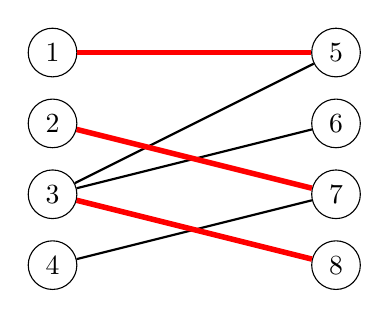
\begin{tikzpicture}[scale=0.60]
\node[draw, circle] (1) at (2,4.5) {1};
\node[draw, circle] (2) at (2,3) {2};
\node[draw, circle] (3) at (2,1.5) {3};
\node[draw, circle] (4) at (2,0) {4};
\node[draw, circle] (5) at (8,4.5) {5};
\node[draw, circle] (6) at (8,3) {6};
\node[draw, circle] (7) at (8,1.5) {7};
\node[draw, circle] (8) at (8,0) {8};

\path[draw,thick,-] (1) -- (5);
\path[draw,thick,-] (2) -- (7);
\path[draw,thick,-] (3) -- (5);
\path[draw,thick,-] (3) -- (6);
\path[draw,thick,-] (3) -- (8);
\path[draw,thick,-] (4) -- (7);

\path[draw=red,thick,-,line width=2pt] (1) -- (5);
\path[draw=red,thick,-,line width=2pt] (2) -- (7);
\path[draw=red,thick,-,line width=2pt] (3) -- (8);
\end{tikzpicture}
\end{center}


このグラフにソースとシンクという2つのノードを新たに加えることで、
二部最大マッチング問題を最大フロー問題に還元することができます。
ソースから各左ノードへ、各右ノードからシンクへのエッジを追加しましょう。
この後、グラフ内の最大流の大きさは、元のグラフの最大マッチングの大きさと等しくなります。

次のようなグラフとします。

\begin{center}
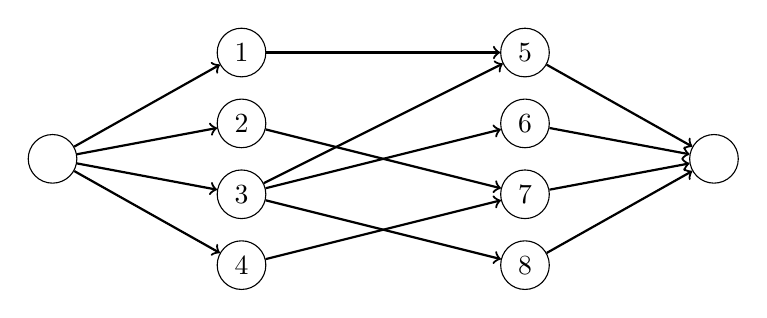
\begin{tikzpicture}[scale=0.60]
\node[draw, circle] (1) at (2,4.5) {1};
\node[draw, circle] (2) at (2,3) {2};
\node[draw, circle] (3) at (2,1.5) {3};
\node[draw, circle] (4) at (2,0) {4};
\node[draw, circle] (5) at (8,4.5) {5};
\node[draw, circle] (6) at (8,3) {6};
\node[draw, circle] (7) at (8,1.5) {7};
\node[draw, circle] (8) at (8,0) {8};

\node[draw, circle] (a) at (-2,2.25) {\phantom{0}};
\node[draw, circle] (b) at (12,2.25) {\phantom{0}};

\path[draw,thick,->] (1) -- (5);
\path[draw,thick,->] (2) -- (7);
\path[draw,thick,->] (3) -- (5);
\path[draw,thick,->] (3) -- (6);
\path[draw,thick,->] (3) -- (8);
\path[draw,thick,->] (4) -- (7);

\path[draw,thick,->] (a) -- (1);
\path[draw,thick,->] (a) -- (2);
\path[draw,thick,->] (a) -- (3);
\path[draw,thick,->] (a) -- (4);
\path[draw,thick,->] (5) -- (b);
\path[draw,thick,->] (6) -- (b);
\path[draw,thick,->] (7) -- (b);
\path[draw,thick,->] (8) -- (b);
\end{tikzpicture}
\end{center}

最大流は以下のようになります。

\begin{center}
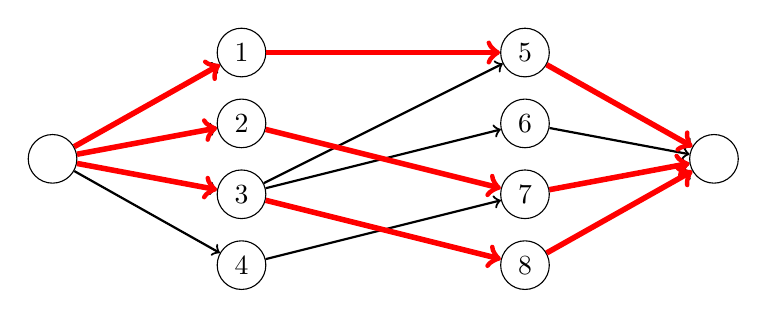
\begin{tikzpicture}[scale=0.60]
\node[draw, circle] (1) at (2,4.5) {1};
\node[draw, circle] (2) at (2,3) {2};
\node[draw, circle] (3) at (2,1.5) {3};
\node[draw, circle] (4) at (2,0) {4};
\node[draw, circle] (5) at (8,4.5) {5};
\node[draw, circle] (6) at (8,3) {6};
\node[draw, circle] (7) at (8,1.5) {7};
\node[draw, circle] (8) at (8,0) {8};

\node[draw, circle] (a) at (-2,2.25) {\phantom{0}};
\node[draw, circle] (b) at (12,2.25) {\phantom{0}};

\path[draw,thick,->] (3) -- (5);
\path[draw,thick,->] (3) -- (6);
\path[draw,thick,->] (4) -- (7);

\path[draw,thick,->] (a) -- (1);
\path[draw,thick,->] (a) -- (2);
\path[draw,thick,->] (a) -- (3);
\path[draw,thick,->] (a) -- (4);
\path[draw,thick,->] (5) -- (b);
\path[draw,thick,->] (6) -- (b);
\path[draw,thick,->] (7) -- (b);
\path[draw,thick,->] (8) -- (b);

\path[draw=red,thick,->,line width=2pt] (1) -- (5);
\path[draw=red,thick,->,line width=2pt] (2) -- (7);
\path[draw=red,thick,->,line width=2pt] (3) -- (8);

\path[draw=red,thick,->,line width=2pt] (a) -- (1);
\path[draw=red,thick,->,line width=2pt] (a) -- (2);
\path[draw=red,thick,->,line width=2pt] (a) -- (3);

\path[draw=red,thick,->,line width=2pt] (5) -- (b);
\path[draw=red,thick,->,line width=2pt] (7) -- (b);
\path[draw=red,thick,->,line width=2pt] (8) -- (b);

\end{tikzpicture}
\end{center}

\subsubsection{ホールの定理 - Hall's theorem}

\index{ホールの定理 - Hall's theorem}
\index{完全マッチング - perfect matching}

\key{ホールの定理 - Hall's theorem} は、
二部グラフがすべての左ノードまたは右ノードを含むマッチングを持つかどうかを調べることができます。
左右のノードの数が同じとき、グラフのすべてのノードを含む\key{完全マッチング}を構成できるかどうかが、
ホールの定理で判定できます。

すべての左ノードを含むマッチングを見つけたいとします。
$X$を任意の左ノードの集合、$f(X)$をその隣接ノードの集合としましょう。
ホールの定理によれば、すべての左ノードを含むマッチングは
、各$X$について$|X| \le |f(X)|$の条件が成立するときに存在します。

ホールの定理を例のグラフで確認します。
まず、$X=\{1,3\}$ とすると、$f(X)=\{5,6,8\}$です。

\begin{center}
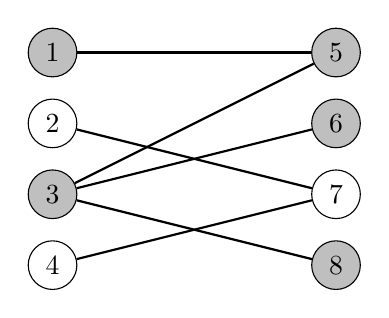
\begin{tikzpicture}[scale=0.60]
\node[draw, circle, fill=lightgray] (1) at (2,4.5) {1};
\node[draw, circle] (2) at (2,3) {2};
\node[draw, circle, fill=lightgray] (3) at (2,1.5) {3};
\node[draw, circle] (4) at (2,0) {4};
\node[draw, circle, fill=lightgray] (5) at (8,4.5) {5};
\node[draw, circle, fill=lightgray] (6) at (8,3) {6};
\node[draw, circle] (7) at (8,1.5) {7};
\node[draw, circle, fill=lightgray] (8) at (8,0) {8};

\path[draw,thick,-] (1) -- (5);
\path[draw,thick,-] (2) -- (7);
\path[draw,thick,-] (3) -- (5);
\path[draw,thick,-] (3) -- (6);
\path[draw,thick,-] (3) -- (8);
\path[draw,thick,-] (4) -- (7);
\end{tikzpicture}
\end{center}

$|X|=2$ and $|f(X)|=3$なので、条件は成り立っています。
次に、$X=\{2,4\}$ で $f(X)=\{7\}$です。

\begin{center}
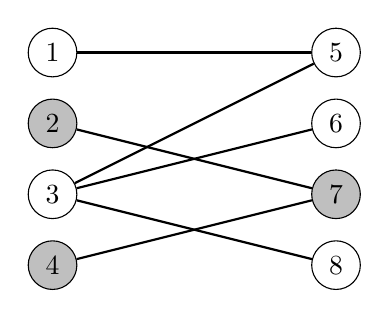
\begin{tikzpicture}[scale=0.60]
\node[draw, circle] (1) at (2,4.5) {1};
\node[draw, circle, fill=lightgray] (2) at (2,3) {2};
\node[draw, circle] (3) at (2,1.5) {3};
\node[draw, circle, fill=lightgray] (4) at (2,0) {4};
\node[draw, circle] (5) at (8,4.5) {5};
\node[draw, circle] (6) at (8,3) {6};
\node[draw, circle, fill=lightgray] (7) at (8,1.5) {7};
\node[draw, circle] (8) at (8,0) {8};

\path[draw,thick,-] (1) -- (5);
\path[draw,thick,-] (2) -- (7);
\path[draw,thick,-] (3) -- (5);
\path[draw,thick,-] (3) -- (6);
\path[draw,thick,-] (3) -- (8);
\path[draw,thick,-] (4) -- (7);
\end{tikzpicture}
\end{center}

この場合、$|X|=2$ ,  $|f(X)|=1$なので、
ホールの定理の条件は成立しません。
つまり、グラフの完全マッチングを形成することはできません。
グラフの最大マッチングは4ではなく3であることがすでに分かってはいますが。

この場合、そのようなマッチングが成立しない理由を集合Xで説明しましょう。
$X$ は $f(X)$ よりも多くのノードを含むので、
$X$のすべてのノードに対応するペアは存在しません。
例えば、上のグラフでは、ノード2とノード4 はともにノード7と接続されて欲しいですが、それは不可能です。

\subsubsection{ケーニヒの定理 - Kőnig's theorem}

\index{ケーニヒの定理 - Kőnig's theorem}
\index{点被覆 - node cover}
\index{最小点被覆 - minimum node cover}

A \key{最小点被覆 - minimum node cover} は、
グラフの各辺が少なくとも1つのエンドポイントを持つようなノードの最小集合です。
一般的なグラフでは、点被覆の最小値を求めることはNP-Hardな問題である。
しかし、グラフが二部グラフであれば、ケーニヒの定理により、
最小点被覆の大きさは最大マッチングと等しくなります。
このため、最大流のアルゴリズムでこれを求めることができます。

では、次のような最大マッチング3のグラフを考えます。

\begin{center}
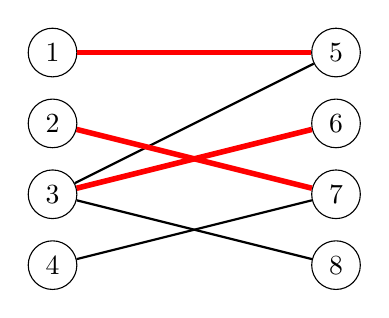
\begin{tikzpicture}[scale=0.60]
\node[draw, circle] (1) at (2,4.5) {1};
\node[draw, circle] (2) at (2,3) {2};
\node[draw, circle] (3) at (2,1.5) {3};
\node[draw, circle] (4) at (2,0) {4};
\node[draw, circle] (5) at (8,4.5) {5};
\node[draw, circle] (6) at (8,3) {6};
\node[draw, circle] (7) at (8,1.5) {7};
\node[draw, circle] (8) at (8,0) {8};

\path[draw,thick,-] (1) -- (5);
\path[draw,thick,-] (2) -- (7);
\path[draw,thick,-] (3) -- (5);
\path[draw,thick,-] (3) -- (6);
\path[draw,thick,-] (3) -- (8);
\path[draw,thick,-] (4) -- (7);

\path[draw=red,thick,-,line width=2pt] (1) -- (5);
\path[draw=red,thick,-,line width=2pt] (2) -- (7);
\path[draw=red,thick,-,line width=2pt] (3) -- (6);
\end{tikzpicture}
\end{center}

ケーニヒの定理から最小点被覆のサイズが3であることが分かります。

\begin{center}
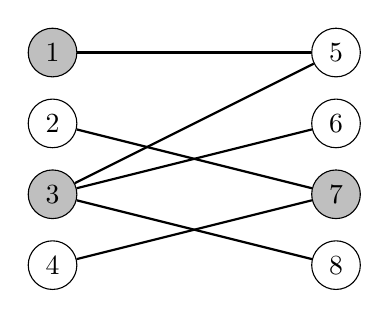
\begin{tikzpicture}[scale=0.60]
\node[draw, circle, fill=lightgray] (1) at (2,4.5) {1};
\node[draw, circle] (2) at (2,3) {2};
\node[draw, circle, fill=lightgray] (3) at (2,1.5) {3};
\node[draw, circle] (4) at (2,0) {4};
\node[draw, circle] (5) at (8,4.5) {5};
\node[draw, circle] (6) at (8,3) {6};
\node[draw, circle, fill=lightgray] (7) at (8,1.5) {7};
\node[draw, circle] (8) at (8,0) {8};

\path[draw,thick,-] (1) -- (5);
\path[draw,thick,-] (2) -- (7);
\path[draw,thick,-] (3) -- (5);
\path[draw,thick,-] (3) -- (6);
\path[draw,thick,-] (3) -- (8);
\path[draw,thick,-] (4) -- (7);
\end{tikzpicture}
\end{center}

\index{独立集合 - independent set}
\index{最大独立集合 - maximum independent set}

最小点被覆に属さないノードは、最大独立集合を形成します。
これは、集合内の2つのノードがエッジで接続されていないようなノードの可能な限り大きな集合である。
繰り返しますが、一般のグラフで最大独立集合を求めるのはNP-Hardな問題ですが、
二部グラフではケーニヒの定理を使って効率的に問題を解くことができます。
例のグラフでは、最大独立集合は次のようになります。

\begin{center}
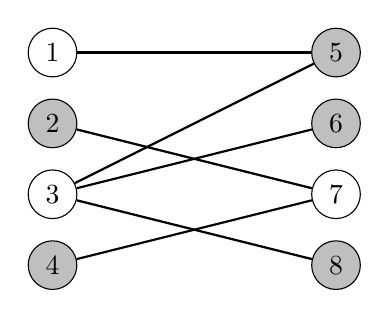
\begin{tikzpicture}[scale=0.60]
\node[draw, circle] (1) at (2,4.5) {1};
\node[draw, circle, fill=lightgray] (2) at (2,3) {2};
\node[draw, circle] (3) at (2,1.5) {3};
\node[draw, circle, fill=lightgray] (4) at (2,0) {4};
\node[draw, circle, fill=lightgray] (5) at (8,4.5) {5};
\node[draw, circle, fill=lightgray] (6) at (8,3) {6};
\node[draw, circle] (7) at (8,1.5) {7};
\node[draw, circle, fill=lightgray] (8) at (8,0) {8};

\path[draw,thick,-] (1) -- (5);
\path[draw,thick,-] (2) -- (7);
\path[draw,thick,-] (3) -- (5);
\path[draw,thick,-] (3) -- (6);
\path[draw,thick,-] (3) -- (8);
\path[draw,thick,-] (4) -- (7);
\end{tikzpicture}
\end{center}

\section{辺被覆 - Path covers}

\index{辺被覆 - path cover}

\key{辺被覆 - path cover} はグラフの各ノードが少なくとも1つのパスに属するようなグラフの
パスの集合のことです。
閉路を含まない有向グラフにおいて、
最小辺被覆を求める問題は、
別のグラフで最大流を求める問題に帰着できることがわかります。

\subsubsection{点素な辺被覆 - Node-disjoint path cover}

In a \key{点素な辺被覆 - node-disjoint path cover},
では、各ノードは正確に1つのパスに属します。
例と して、次のようなグラフを考えてみよう。

\begin{center}
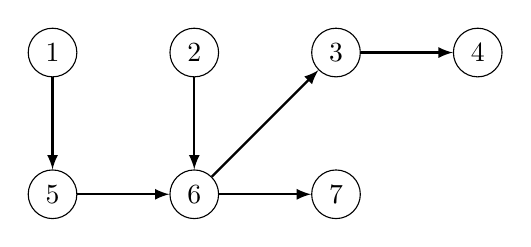
\begin{tikzpicture}[scale=0.9]
\node[draw, circle] (1) at (0,0) {1};
\node[draw, circle] (2) at (2,0) {2};
\node[draw, circle] (3) at (4,0) {3};
\node[draw, circle] (4) at (6,0) {4};
\node[draw, circle] (5) at (0,-2) {5};
\node[draw, circle] (6) at (2,-2) {6};
\node[draw, circle] (7) at (4,-2) {7};

\path[draw,thick,->,>=latex] (1) -- (5);
\path[draw,thick,->,>=latex] (2) -- (6);
\path[draw,thick,->,>=latex] (3) -- (4);
\path[draw,thick,->,>=latex] (5) -- (6);
\path[draw,thick,->,>=latex] (6) -- (3);
\path[draw,thick,->,>=latex] (6) -- (7);
\end{tikzpicture}
\end{center}


このグラフの最小の点素な辺被覆は、3つのパスから構成されます。

\begin{center}
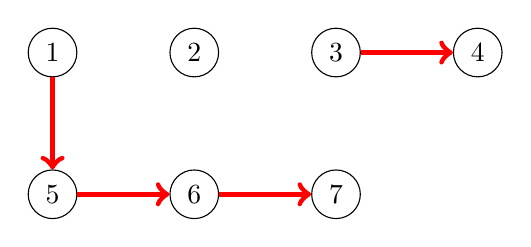
\begin{tikzpicture}[scale=0.9]
\node[draw, circle] (1) at (0,0) {1};
\node[draw, circle] (2) at (2,0) {2};
\node[draw, circle] (3) at (4,0) {3};
\node[draw, circle] (4) at (6,0) {4};
\node[draw, circle] (5) at (0,-2) {5};
\node[draw, circle] (6) at (2,-2) {6};
\node[draw, circle] (7) at (4,-2) {7};

\path[draw=red,thick,->,line width=2pt] (1) -- (5);
\path[draw=red,thick,->,line width=2pt] (5) -- (6);
\path[draw=red,thick,->,line width=2pt] (6) -- (7);
\path[draw=red,thick,->,line width=2pt] (3) -- (4);
\end{tikzpicture}
\end{center}

なお、ノード2しか含まない集合があるようにパスに点が含まれないこともあります。

ここで、元のグラフの各ノードを左ノードと右ノードの2つのノードで表現したマッチンググラフを構築することで、
最小の点素な辺被覆を求めることができます。
元のグラフに左ノードから右ノードへのエッジがある場合、そのエッジはマッチンググラフにも存在します。
また、マッチンググラフにはソースとシンクがあり、ソースからすべての左ノードへ、
すべての右ノードからシンクへのエッジが存在する。

この結果得られたグラフの最大マッチングは、
元のグラフの最小の点素な辺被覆に対応します。
例えば、上記のグラフに対する以下のマッチンググラフは、
サイズ4の最大マッチングを含んでいます。

\begin{center}
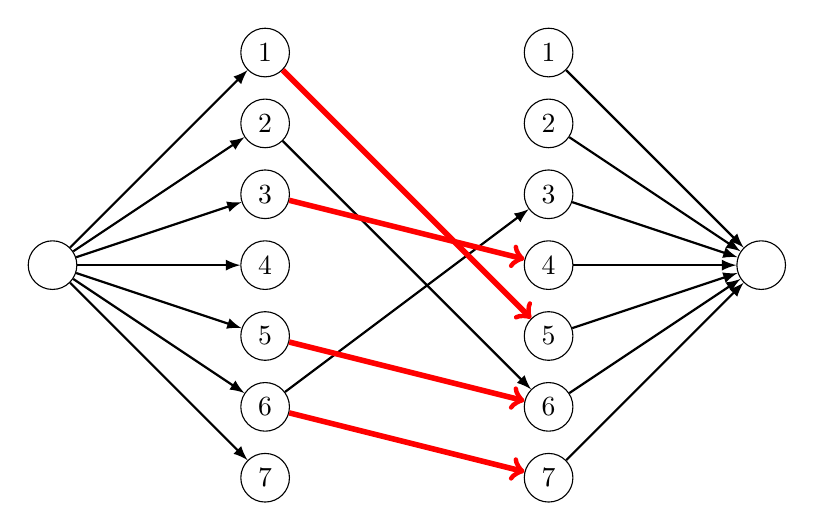
\begin{tikzpicture}[scale=0.9]
\node[draw, circle] (1a) at (0,6) {1};
\node[draw, circle] (2a) at (0,5) {2};
\node[draw, circle] (3a) at (0,4) {3};
\node[draw, circle] (4a) at (0,3) {4};
\node[draw, circle] (5a) at (0,2) {5};
\node[draw, circle] (6a) at (0,1) {6};
\node[draw, circle] (7a) at (0,0) {7};

\node[draw, circle] (1b) at (4,6) {1};
\node[draw, circle] (2b) at (4,5) {2};
\node[draw, circle] (3b) at (4,4) {3};
\node[draw, circle] (4b) at (4,3) {4};
\node[draw, circle] (5b) at (4,2) {5};
\node[draw, circle] (6b) at (4,1) {6};
\node[draw, circle] (7b) at (4,0) {7};

\node[draw, circle] (a) at (-3,3) {\phantom{0}};
\node[draw, circle] (b) at (7,3) {\phantom{0}};

%\path[draw,thick,->,>=latex] (1a) -- (5b);
\path[draw,thick,->,>=latex] (2a) -- (6b);
%\path[draw,thick,->,>=latex] (3a) -- (4b);
%\path[draw,thick,->,>=latex] (5a) -- (6b);
\path[draw,thick,->,>=latex] (6a) -- (3b);
%\path[draw,thick,->,>=latex] (6a) -- (7b);

\path[draw,thick,->,>=latex] (a) -- (1a);
\path[draw,thick,->,>=latex] (a) -- (2a);
\path[draw,thick,->,>=latex] (a) -- (3a);
\path[draw,thick,->,>=latex] (a) -- (4a);
\path[draw,thick,->,>=latex] (a) -- (5a);
\path[draw,thick,->,>=latex] (a) -- (6a);
\path[draw,thick,->,>=latex] (a) -- (7a);

\path[draw,thick,->,>=latex] (1b) -- (b);
\path[draw,thick,->,>=latex] (2b) -- (b);
\path[draw,thick,->,>=latex] (3b) -- (b);
\path[draw,thick,->,>=latex] (4b) -- (b);
\path[draw,thick,->,>=latex] (5b) -- (b);
\path[draw,thick,->,>=latex] (6b) -- (b);
\path[draw,thick,->,>=latex] (7b) -- (b);

\path[draw=red,thick,->,line width=2pt] (1a) -- (5b);
\path[draw=red,thick,->,line width=2pt] (5a) -- (6b);
\path[draw=red,thick,->,line width=2pt] (6a) -- (7b);
\path[draw=red,thick,->,line width=2pt] (3a) -- (4b);

\end{tikzpicture}
\end{center}

マッチンググラフの最大マッチングの各エッジは、
元のグラフの最小の点素な辺被覆のエッジに対応します。
したがって、最小の点素な辺被覆の最小サイズは$n - c$といえます。
ここで$n$は元グラフのノード数、$c$は最大マッチングのサイズである。

\subsubsection{一般的な辺被覆 - General path cover}

\key{一般的な辺被覆 - general path cover} は
1つのノードが複数のパスに属することができる辺被覆のことです。
1つのノードは複数回パスで使われることがあるため,
最小の一般的な辺被覆は
最小の点素な辺被覆より小さくなることがあります。
先ほどのグラフを例にとります。

\begin{center}
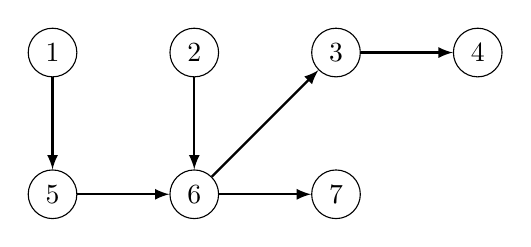
\begin{tikzpicture}[scale=0.9]
\node[draw, circle] (1) at (0,0) {1};
\node[draw, circle] (2) at (2,0) {2};
\node[draw, circle] (3) at (4,0) {3};
\node[draw, circle] (4) at (6,0) {4};
\node[draw, circle] (5) at (0,-2) {5};
\node[draw, circle] (6) at (2,-2) {6};
\node[draw, circle] (7) at (4,-2) {7};

\path[draw,thick,->,>=latex] (1) -- (5);
\path[draw,thick,->,>=latex] (2) -- (6);
\path[draw,thick,->,>=latex] (3) -- (4);
\path[draw,thick,->,>=latex] (5) -- (6);
\path[draw,thick,->,>=latex] (6) -- (3);
\path[draw,thick,->,>=latex] (6) -- (7);
\end{tikzpicture}
\end{center}

このグラフにおける最小の一般的な辺被覆は、
2つの経路で作れます。まず1つ目は

\begin{center}
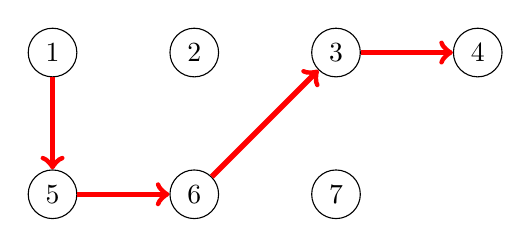
\begin{tikzpicture}[scale=0.9]
\node[draw, circle] (1) at (0,0) {1};
\node[draw, circle] (2) at (2,0) {2};
\node[draw, circle] (3) at (4,0) {3};
\node[draw, circle] (4) at (6,0) {4};
\node[draw, circle] (5) at (0,-2) {5};
\node[draw, circle] (6) at (2,-2) {6};
\node[draw, circle] (7) at (4,-2) {7};

\path[draw=red,thick,->,line width=2pt] (1) -- (5);
\path[draw=red,thick,->,line width=2pt] (5) -- (6);
\path[draw=red,thick,->,line width=2pt] (6) -- (3);
\path[draw=red,thick,->,line width=2pt] (3) -- (4);
\end{tikzpicture}
\end{center}
次に2つ目は、
\begin{center}
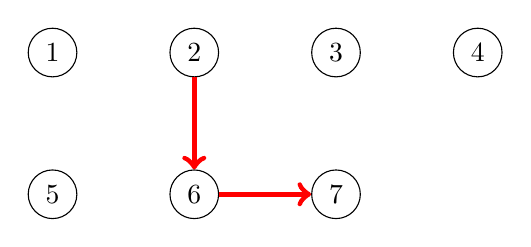
\begin{tikzpicture}[scale=0.9]
\node[draw, circle] (1) at (0,0) {1};
\node[draw, circle] (2) at (2,0) {2};
\node[draw, circle] (3) at (4,0) {3};
\node[draw, circle] (4) at (6,0) {4};
\node[draw, circle] (5) at (0,-2) {5};
\node[draw, circle] (6) at (2,-2) {6};
\node[draw, circle] (7) at (4,-2) {7};

\path[draw=red,thick,->,line width=2pt] (2) -- (6);
\path[draw=red,thick,->,line width=2pt] (6) -- (7);
\end{tikzpicture}
\end{center}


最小の一般的な辺被覆は、最小の点素な辺被覆とほぼ同様に求めることができます。
マッチンググラフに新しい辺をいくつか追加し,
元のグラフに$a$から$b$への経路があるときに必ず辺$a \rightarrow b$が存在するようにすればよいです
(これはいくつかの辺 を経由する場合もある)。

上記のグラフのマッチンググラフは次のようになる。
\begin{center}
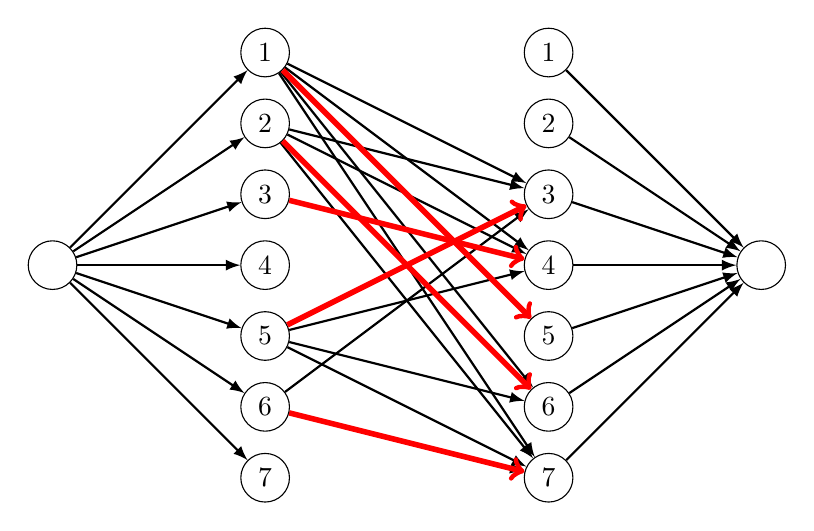
\begin{tikzpicture}[scale=0.9]
\node[draw, circle] (1a) at (0,6) {1};
\node[draw, circle] (2a) at (0,5) {2};
\node[draw, circle] (3a) at (0,4) {3};
\node[draw, circle] (4a) at (0,3) {4};
\node[draw, circle] (5a) at (0,2) {5};
\node[draw, circle] (6a) at (0,1) {6};
\node[draw, circle] (7a) at (0,0) {7};

\node[draw, circle] (1b) at (4,6) {1};
\node[draw, circle] (2b) at (4,5) {2};
\node[draw, circle] (3b) at (4,4) {3};
\node[draw, circle] (4b) at (4,3) {4};
\node[draw, circle] (5b) at (4,2) {5};
\node[draw, circle] (6b) at (4,1) {6};
\node[draw, circle] (7b) at (4,0) {7};

\node[draw, circle] (a) at (-3,3) {\phantom{0}};
\node[draw, circle] (b) at (7,3) {\phantom{0}};


%\path[draw,thick,->,>=latex] (1a) -- (5b);
\path[draw,thick,->,>=latex] (1a) -- (6b);
\path[draw,thick,->,>=latex] (1a) -- (7b);
\path[draw,thick,->,>=latex] (1a) -- (3b);
\path[draw,thick,->,>=latex] (1a) -- (4b);
\path[draw,thick,->,>=latex] (5a) -- (6b);
\path[draw,thick,->,>=latex] (5a) -- (7b);
%\path[draw,thick,->,>=latex] (5a) -- (3b);
\path[draw,thick,->,>=latex] (5a) -- (4b);
\path[draw,thick,->,>=latex] (6a) -- (7b);
%\path[draw,thick,->,>=latex] (6a) -- (7b);
\path[draw,thick,->,>=latex] (6a) -- (3b);
%\path[draw,thick,->,>=latex] (3a) -- (4b);
%\path[draw,thick,->,>=latex] (2a) -- (6b);
\path[draw,thick,->,>=latex] (2a) -- (7b);
\path[draw,thick,->,>=latex] (2a) -- (3b);
\path[draw,thick,->,>=latex] (2a) -- (4b);


\path[draw,thick,->,>=latex] (a) -- (1a);
\path[draw,thick,->,>=latex] (a) -- (2a);
\path[draw,thick,->,>=latex] (a) -- (3a);
\path[draw,thick,->,>=latex] (a) -- (4a);
\path[draw,thick,->,>=latex] (a) -- (5a);
\path[draw,thick,->,>=latex] (a) -- (6a);
\path[draw,thick,->,>=latex] (a) -- (7a);

\path[draw,thick,->,>=latex] (1b) -- (b);
\path[draw,thick,->,>=latex] (2b) -- (b);
\path[draw,thick,->,>=latex] (3b) -- (b);
\path[draw,thick,->,>=latex] (4b) -- (b);
\path[draw,thick,->,>=latex] (5b) -- (b);
\path[draw,thick,->,>=latex] (6b) -- (b);
\path[draw,thick,->,>=latex] (7b) -- (b);

\path[draw=red,thick,->,line width=2pt] (1a) -- (5b);
\path[draw=red,thick,->,line width=2pt] (5a) -- (3b);
\path[draw=red,thick,->,line width=2pt] (3a) -- (4b);
\path[draw=red,thick,->,line width=2pt] (2a) -- (6b);
\path[draw=red,thick,->,line width=2pt] (6a) -- (7b);


% \path[draw=red,thick,->,line width=2pt] (1a) -- (6b);
% \path[draw=red,thick,->,line width=2pt] (1a) -- (7b);
% \path[draw=red,thick,->,line width=2pt] (1a) -- (3b);
% \path[draw=red,thick,->,line width=2pt] (1a) -- (4b);
% \path[draw=red,thick,->,line width=2pt] (5a) -- (6b);
% \path[draw=red,thick,->,line width=2pt] (5a) -- (7b);
% \path[draw=red,thick,->,line width=2pt] (5a) -- (3b);
% \path[draw=red,thick,->,line width=2pt] (5a) -- (4b);
% \path[draw=red,thick,->,line width=2pt] (6a) -- (7b);
% \path[draw=red,thick,->,line width=2pt] (6a) -- (7b);
% \path[draw=red,thick,->,line width=2pt] (6a) -- (3b);
% \path[draw=red,thick,->,line width=2pt] (3a) -- (4b);
% \path[draw=red,thick,->,line width=2pt] (2a) -- (6b);
% \path[draw=red,thick,->,line width=2pt] (2a) -- (7b);
% \path[draw=red,thick,->,line width=2pt] (2a) -- (3b);
% \path[draw=red,thick,->,line width=2pt] (2a) -- (4b);

\end{tikzpicture}
\end{center}

\subsubsection{ディルワースの定理 - Dilworth's theorem}

\index{ディルワースの定理 - Dilworth's theorem}
\index{反鎖 - antichain}

\key{反鎖 - antichain} とは、グラフの辺をを使い、
どのノードからも他のノードへの経路が存在しないようなノードの集合のことである。
\key{ディルワースの定理 - Dilworth's theorem}では、
閉路の存在しない有向グラフにおいて、
最小の一般的な辺被覆の大きさは最大の 反鎖の大きさに等しいとする。
例えば、以下のグラフでは、ノード3と7が反鎖を形成しています。

\begin{center}
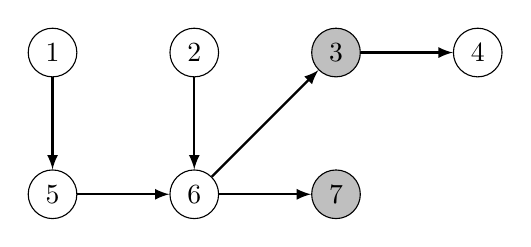
\begin{tikzpicture}[scale=0.9]
\node[draw, circle] (1) at (0,0) {1};
\node[draw, circle] (2) at (2,0) {2};
\node[draw, circle, fill=lightgray] (3) at (4,0) {3};
\node[draw, circle] (4) at (6,0) {4};
\node[draw, circle] (5) at (0,-2) {5};
\node[draw, circle] (6) at (2,-2) {6};
\node[draw, circle, fill=lightgray] (7) at (4,-2) {7};

\path[draw,thick,->,>=latex] (1) -- (5);
\path[draw,thick,->,>=latex] (2) -- (6);
\path[draw,thick,->,>=latex] (3) -- (4);
\path[draw,thick,->,>=latex] (5) -- (6);
\path[draw,thick,->,>=latex] (6) -- (3);
\path[draw,thick,->,>=latex] (6) -- (7);
\end{tikzpicture}
\end{center}


これは最大反鎖となります。
3つのノードを含むような反鎖は構成できないからです。
このグラフの最小の一般的な辺被覆の大きさは,2つのパスからなることは先に確認しました。
